\renewcommand{\theequation}{\theenumi}
\begin{enumerate}[label=\thesection.\arabic*.,ref=\thesection.\theenumi]
\numberwithin{equation}{enumi}

\item (a) To find p(0) we substitute 0 in place of the variable y in p(y). Similarly we find p(1) and p(2)
\begin{align}
\label{eq:conic1a}
 p(y) = y^{2}
\\
\implies p(0) =0
\\
p(1) = 1
\\
p(2) = 4
\end{align}
The following code sketches the graph of \ref{eq:conic1a} in figure \ref{fig:conic1a}
\begin{lstlisting}
codes/conic1/conic1a.py
\end{lstlisting}
\begin{figure}[!ht]
\centering
\includegraphics[width=\columnwidth]{./codes/conic1/pyfigs/conic1a.eps}
\caption{Graph of p(y)}
\label{fig:conic1a}
\end{figure}


\item (b)Similarly we find p(0), p(1) and p(2) of p(x) by replacing x
\begin{align}
\label{eq:conic1b}
 p(x) = \brak{x-1}\brak{x+1}
\\
\implies p(0) =-1
\\
p(1) = 0
\\
p(2) = 3
\end{align}
The following code sketches the graph of \ref{eq:conic1b} in figure \ref{fig:conic1b}
\begin{lstlisting}
codes/conic1/conic1b.py
\end{lstlisting}
\begin{figure}[!ht]
\centering
\includegraphics[width=\columnwidth]{./codes/conic1/pyfigs/conic1b.eps}
\caption{Graph of p(x)}
\label{fig:conic1b}
\end{figure}

\end{enumerate}
